\chapter{Model 7: Quantile Regression}\label{ch:model7}

% Include the dynamic values from model calibration
% Model 7 Calibrated Values
% Generated: 2025-10-07 09:39:44.326058
% Model: Quantile Regression

% Core Metrics
\renewcommand{\ModelSevenRSquaredTrain}{0.2524}
\renewcommand{\ModelSevenRSquaredTest}{0.2246}
\renewcommand{\ModelSevenRMSETrain}{38,160}
\renewcommand{\ModelSevenRMSETest}{38,456}
\renewcommand{\ModelSevenMAETrain}{27,199}
\renewcommand{\ModelSevenMAETest}{27,562}
\renewcommand{\ModelSevenMAPETrain}{84.7}
\renewcommand{\ModelSevenMAPETest}{85.3}
\renewcommand{\ModelSevenCVMean}{0.2516}
\renewcommand{\ModelSevenCVStd}{0.0147}
\renewcommand{\ModelSevenWithinOneK}{3.7}
\renewcommand{\ModelSevenWithinTwoK}{7.0}
\renewcommand{\ModelSevenWithinFiveK}{15.1}
\renewcommand{\ModelSevenWithinTenK}{27.5}
\renewcommand{\ModelSevenWithinTwentyK}{49.1}
\renewcommand{\ModelSevenTrainingSamples}{53,812}
\renewcommand{\ModelSevenTestSamples}{13,453}

% Subgroup Metrics
\renewcommand{\ModelSevenSubgrouplivingFHN}{11,666}
\renewcommand{\ModelSevenSubgrouplivingFHRSquared}{0.228}
\renewcommand{\ModelSevenSubgrouplivingFHRMSE}{39,026}
\renewcommand{\ModelSevenSubgrouplivingFHBias}{-6,165}
\renewcommand{\ModelSevenSubgrouplivingILSLN}{1,787}
\renewcommand{\ModelSevenSubgrouplivingILSLRSquared}{0.199}
\renewcommand{\ModelSevenSubgrouplivingILSLRMSE}{34,506}
\renewcommand{\ModelSevenSubgrouplivingILSLBias}{-3,258}
\renewcommand{\ModelSevenSubgroupageAgeUnderTwentyOneN}{1,300}
\renewcommand{\ModelSevenSubgroupageAgeUnderTwentyOneRSquared}{0.017}
\renewcommand{\ModelSevenSubgroupageAgeUnderTwentyOneRMSE}{40,058}
\renewcommand{\ModelSevenSubgroupageAgeUnderTwentyOneBias}{-14,382}
\renewcommand{\ModelSevenSubgroupageAgeTwentyOneToThirtyN}{3,770}
\renewcommand{\ModelSevenSubgroupageAgeTwentyOneToThirtyRSquared}{0.176}
\renewcommand{\ModelSevenSubgroupageAgeTwentyOneToThirtyRMSE}{43,445}
\renewcommand{\ModelSevenSubgroupageAgeTwentyOneToThirtyBias}{-7,298}
\renewcommand{\ModelSevenSubgroupageAgeThirtyOnePlusN}{8,383}
\renewcommand{\ModelSevenSubgroupageAgeThirtyOnePlusRSquared}{0.259}
\renewcommand{\ModelSevenSubgroupageAgeThirtyOnePlusRMSE}{35,716}
\renewcommand{\ModelSevenSubgroupageAgeThirtyOnePlusBias}{-3,762}
\renewcommand{\ModelSevenSubgroupcostQOneLowN}{3,365}
\renewcommand{\ModelSevenSubgroupcostQOneLowRSquared}{-10.000}
\renewcommand{\ModelSevenSubgroupcostQOneLowRMSE}{33,109}
\renewcommand{\ModelSevenSubgroupcostQOneLowBias}{+25,519}
\renewcommand{\ModelSevenSubgroupcostQTwoN}{3,362}
\renewcommand{\ModelSevenSubgroupcostQTwoRSquared}{-7.118}
\renewcommand{\ModelSevenSubgroupcostQTwoRMSE}{20,447}
\renewcommand{\ModelSevenSubgroupcostQTwoBias}{+10,411}
\renewcommand{\ModelSevenSubgroupcostQThreeN}{3,363}
\renewcommand{\ModelSevenSubgroupcostQThreeRSquared}{-3.662}
\renewcommand{\ModelSevenSubgroupcostQThreeRMSE}{24,857}
\renewcommand{\ModelSevenSubgroupcostQThreeBias}{-12,991}
\renewcommand{\ModelSevenSubgroupcostQFourHighN}{3,363}
\renewcommand{\ModelSevenSubgroupcostQFourHighRSquared}{-2.124}
\renewcommand{\ModelSevenSubgroupcostQFourHighRMSE}{61,508}
\renewcommand{\ModelSevenSubgroupcostQFourHighBias}{-46,070}

% Variance Metrics
\renewcommand{\ModelSevenCVActual}{1.011}
\renewcommand{\ModelSevenCVPredicted}{0.676}
\renewcommand{\ModelSevenPredictionInterval}{149,036}
\renewcommand{\ModelSevenBudgetActualCorr}{0.499}
\renewcommand{\ModelSevenQuarterlyVariance}{88.0}
\renewcommand{\ModelSevenAnnualAdjustmentRate}{92.7}

% Population Scenarios
\renewcommand{\ModelSevenPopcurrentbaselineClients}{32,085}
\renewcommand{\ModelSevenPopcurrentbaselineAvgAlloc}{37,400}
\renewcommand{\ModelSevenPopcurrentbaselineWaitlistChange}{+0}
\renewcommand{\ModelSevenPopcurrentbaselineWaitlistPct}{+0.0}
\renewcommand{\ModelSevenPopmodelbalancedClients}{32,726}
\renewcommand{\ModelSevenPopmodelbalancedAvgAlloc}{36,652}
\renewcommand{\ModelSevenPopmodelbalancedWaitlistChange}{+641}
\renewcommand{\ModelSevenPopmodelbalancedWaitlistPct}{+2.0}
\renewcommand{\ModelSevenPopmodelefficiencyClients}{33,689}
\renewcommand{\ModelSevenPopmodelefficiencyAvgAlloc}{35,530}
\renewcommand{\ModelSevenPopmodelefficiencyWaitlistChange}{+1,604}
\renewcommand{\ModelSevenPopmodelefficiencyWaitlistPct}{+5.0}
\renewcommand{\ModelSevenPopcategoryfocusedClients}{27,272}
\renewcommand{\ModelSevenPopcategoryfocusedAvgAlloc}{44,132}
\renewcommand{\ModelSevenPopcategoryfocusedWaitlistChange}{-4,812}
\renewcommand{\ModelSevenPopcategoryfocusedWaitlistPct}{-15.0}
\renewcommand{\ModelSevenPoppopulationmaximizedClients}{36,897}
\renewcommand{\ModelSevenPoppopulationmaximizedAvgAlloc}{32,538}
\renewcommand{\ModelSevenPoppopulationmaximizedWaitlistChange}{+4,812}
\renewcommand{\ModelSevenPoppopulationmaximizedWaitlistPct}{+15.0}

% ============================================================================
% Model 7 Quantile-Specific Values
% ============================================================================
\renewcommand{\ModelSevenQuantileTenRSquared}{0.7029}
\renewcommand{\ModelSevenQuantileTwentyFiveRSquared}{0.3696}
\renewcommand{\ModelSevenQuantileFiftyRSquared}{0.2173}
\renewcommand{\ModelSevenQuantileSeventyFiveRSquared}{0.4092}
\renewcommand{\ModelSevenQuantileNinetyRSquared}{0.6856}
\renewcommand{\ModelSevenPredictionIntervalWidth}{86,336}
\renewcommand{\ModelSevenQuantileSpread}{1.10}
\renewcommand{\ModelSevenQuantileMonotonicity}{98.8}
\renewcommand{\ModelSevenRegulatoryCompliant}{No}
\renewcommand{\ModelSevenRegulatoryWarning}{Produces distributions, not single allocations. Violates F.S. 393.0662.}
\renewcommand{\ModelSevenDeploymentStatus}{Research Only}
\renewcommand{\ModelSevenFatalFlaw}{Produces distributions not single amounts}
\renewcommand{\ModelSevenTransformation}{sqrt}
\renewcommand{\ModelSevenNumFeatures}{23}
\renewcommand{\ModelSevenCVFolds}{10}
\renewcommand{\ModelSevenCVMin}{0.2200}
\renewcommand{\ModelSevenCVMax}{0.2745}


\section{Executive Summary}

Model 7 employs quantile regression to model multiple percentiles of the expenditure distribution simultaneously. While this approach provides superior uncertainty quantification and complete robustness to outliers, it produces a \textbf{distribution of potential allocations rather than the single deterministic amount required by F.S. 393.0662 and F.A.C. 65G-4.0214}. Therefore, this model is \textbf{suitable for research and risk analysis only}, not for production budget allocation.

\subsection{Key Findings}
\begin{itemize}
    \item Median regression achieves $R^2$ = \ModelSevenRSquaredTest{} with RMSE = \$\ModelSevenRMSETest{}
    \item 10th percentile $R^2$ = \ModelSevenQuantileTenRSquared{}
    \item 90th percentile $R^2$ = \ModelSevenQuantileNinetyRSquared{}
    \item Average 80\% prediction interval width: \$\ModelSevenPredictionIntervalWidth{}
    \item Quantile monotonicity maintained in \ModelSevenQuantileMonotonicity{}\% of cases
    \item \textcolor{red}{Regulatory Compliant: \ModelSevenRegulatoryCompliant{}}
\end{itemize}

\section{Algorithm Documentation}

\subsection{Mathematical Specification}

Quantile regression models the $\tau$-th conditional quantile of the response variable:

For quantile $\tau \in (0,1)$:
\begin{equation}
Q_{\tau}(\sqrt{Y_i} | X_i) = \beta_0(\tau) + \sum_{j=1}^{22} \beta_j(\tau) X_{ij}
\end{equation}

The model minimizes the asymmetric check function:
\begin{equation}
\min_{\beta(\tau)} \sum_{i=1}^n \rho_\tau\left(\sqrt{Y_i} - \beta_0(\tau) - \sum_{j=1}^{22} \beta_j(\tau) X_{ij}\right)
\end{equation}

where the check function is defined as:
\begin{equation}
\rho_\tau(u) = u(\tau - \mathbb{I}(u < 0)) = \begin{cases}
\tau u & \text{if } u \geq 0 \\
(\tau - 1) u & \text{if } u < 0
\end{cases}
\end{equation}

\subsection{Multiple Quantile Estimation}

The model estimates five primary quantiles:
\begin{itemize}
    \item $\tau = 0.10$: 10th percentile (minimum needs baseline)
    \item $\tau = 0.25$: 25th percentile (lower quartile)
    \item $\tau = 0.50$: 50th percentile (median, primary estimate)
    \item $\tau = 0.75$: 75th percentile (upper quartile)
    \item $\tau = 0.90$: 90th percentile (high needs ceiling)
\end{itemize}

\subsection{Feature Set}

Model 7 uses the standard 22-feature configuration:
\begin{itemize}
    \item 5 living setting indicators (ILSL, RH1--RH4; FH as reference)
    \item 2 age group indicators (21--30, 31+; under 21 as reference)
    \item 10 individual QSI questions (Q16, Q18, Q20, Q21, Q23, Q28, Q33, Q34, Q36, Q43)
    \item 2 summary scores (BSum, FSum)
    \item 3 primary disability indicators
\end{itemize}

\section{Accuracy and Reliability}

\subsection{Core Performance Metrics}

\begin{table}[h]
\centering
\caption{Model 7 Performance -- Median Regression Focus}
\begin{tabular}{lcc}
\toprule
\textbf{Metric} & \textbf{Training} & \textbf{Test} \\
\midrule
$R^2$ Score & \ModelSevenRSquaredTrain{} & \ModelSevenRSquaredTest{} \\
RMSE & \$\ModelSevenRMSETrain{} & \$\ModelSevenRMSETest{} \\
MAE & \$\ModelSevenMAETrain{} & \$\ModelSevenMAETest{} \\
MAPE & \ModelSevenMAPETrain{}\% & \ModelSevenMAPETest{}\% \\
Cross-Validation $R^2$ & \multicolumn{2}{c}{\ModelSevenCVMean{} $\pm$ \ModelSevenCVStd{}} \\
\bottomrule
\end{tabular}
\end{table}

\subsection{Quantile-Specific Performance}

\begin{table}[h]
\centering
\caption{Performance Across Quantiles}
\begin{tabular}{lccc}
\toprule
\textbf{Quantile} & \textbf{Pseudo-$R^2$} & \textbf{Interpretation} \\
\midrule
0.10 (10th percentile) & \ModelSevenQuantileTenRSquared{} & Minimum needs \\
0.50 (Median) & \ModelSevenRSquaredTest{} & Central tendency \\
0.90 (90th percentile) & \ModelSevenQuantileNinetyRSquared{} & High needs \\
\bottomrule
\end{tabular}
\end{table}

\subsection{Prediction Accuracy Thresholds}

\begin{table}[h]
\centering
\caption{Percentage Within Dollar Thresholds -- Test Set}
\begin{tabular}{lc}
\toprule
\textbf{Threshold} & \textbf{Percentage Within} \\
\midrule
Within \$1,000 & \ModelSevenWithinOneK{}\% \\
Within \$2,000 & \ModelSevenWithinTwoK{}\% \\
Within \$5,000 & \ModelSevenWithinFiveK{}\% \\
Within \$10,000 & \ModelSevenWithinTenK{}\% \\
Within \$20,000 & \ModelSevenWithinTwentyK{}\% \\
\bottomrule
\end{tabular}
\end{table}

\section{Robustness Analysis}

\subsection{Complete Outlier Robustness}

Quantile regression, particularly median regression, is \textbf{completely robust} to outliers:
\begin{itemize}
    \item No outlier removal required (uses 100\% of data)
    \item Median regression has 50\% breakdown point
    \item Influence of extreme values naturally bounded
    \item Training samples used: \ModelSevenTrainingSamples{}
    \item Test samples used: \ModelSevenTestSamples{}
\end{itemize}

\subsection{Heteroscedasticity Handling}

\begin{itemize}
    \item Average 80\% prediction interval width: \$\ModelSevenPredictionIntervalWidth{}
    \item Quantile spread ratio (Q90/Q10): \ModelSevenQuantileSpread{}
    \item Naturally adapts interval width to cost level
    \item No constant variance assumption required
\end{itemize}

\section{Subgroup Performance Analysis}

\begin{table}[h]
\centering
\caption{Median Regression Performance by Subgroup}
\begin{tabular}{lcccc}
\toprule
\textbf{Subgroup} & \textbf{N} & \textbf{$R^2$} & \textbf{RMSE} & \textbf{Bias} \\
\midrule
\multicolumn{5}{l}{\textit{By Living Setting}} \\
Family Home & \ModelSevenSubgrouplivingFHN{} & \ModelSevenSubgrouplivingFHRSquared{} & \$\ModelSevenSubgrouplivingFHRMSE{} & \$\ModelSevenSubgrouplivingFHBias{} \\
ILSL & \ModelSevenSubgrouplivingILSLN{} & \ModelSevenSubgrouplivingILSLRSquared{} & \$\ModelSevenSubgrouplivingILSLRMSE{} & \$\ModelSevenSubgrouplivingILSLBias{} \\
RH (1-4) & \ModelSevenSubgrouplivingRHOneToFourN{} & \ModelSevenSubgrouplivingRHOneToFourRSquared{} & \$\ModelSevenSubgrouplivingRHOneToFourRMSE{} & \$\ModelSevenSubgrouplivingRHOneToFourBias{} \\
\midrule
\multicolumn{5}{l}{\textit{By Age Group}} \\
Under 21 & \ModelSevenSubgroupageAgeUnderTwentyOneN{} & \ModelSevenSubgroupageAgeUnderTwentyOneRSquared{} & \$\ModelSevenSubgroupageAgeUnderTwentyOneRMSE{} & \$\ModelSevenSubgroupageAgeUnderTwentyOneBias{} \\
21--30 & \ModelSevenSubgroupageAgeTwentyOneToThirtyN{} & \ModelSevenSubgroupageAgeTwentyOneToThirtyRSquared{} & \$\ModelSevenSubgroupageAgeTwentyOneToThirtyRMSE{} & \$\ModelSevenSubgroupageAgeTwentyOneToThirtyBias{} \\
31+ & \ModelSevenSubgroupageAgeThirtyOnePlusN{} & \ModelSevenSubgroupageAgeThirtyOnePlusRSquared{} & \$\ModelSevenSubgroupageAgeThirtyOnePlusRMSE{} & \$\ModelSevenSubgroupageAgeThirtyOnePlusBias{} \\
\midrule
\multicolumn{5}{l}{\textit{By Cost Quartile}} \\
Q1 (Lowest) & \ModelSevenSubgroupcostQOneLowN{} & \ModelSevenSubgroupcostQOneLowRSquared{} & \$\ModelSevenSubgroupcostQOneLowRMSE{} & \$\ModelSevenSubgroupcostQOneLowBias{} \\
Q2 & \ModelSevenSubgroupcostQTwoN{} & \ModelSevenSubgroupcostQTwoRSquared{} & \$\ModelSevenSubgroupcostQTwoRMSE{} & \$\ModelSevenSubgroupcostQTwoBias{} \\
Q3 & \ModelSevenSubgroupcostQThreeN{} & \ModelSevenSubgroupcostQThreeRSquared{} & \$\ModelSevenSubgroupcostQThreeRMSE{} & \$\ModelSevenSubgroupcostQThreeBias{} \\
Q4 (Highest) & \ModelSevenSubgroupcostQFourHighN{} & \ModelSevenSubgroupcostQFourHighRSquared{} & \$\ModelSevenSubgroupcostQFourHighRMSE{} & \$\ModelSevenSubgroupcostQFourHighBias{} \\
\bottomrule
\end{tabular}
\end{table}

\section{Variance and Stability Metrics}

\begin{table}[h]
\centering
\caption{Variance Metrics -- Model 7 vs Current}
\begin{tabular}{lcc}
\toprule
\textbf{Metric} & \textbf{Current Model 5b} & \textbf{Model 7 (Median)} \\
\midrule
Coefficient of Variation (Actual) & [baseline] & \ModelSevenCVActual{} \\
Coefficient of Variation (Predicted) & [baseline] & \ModelSevenCVPredicted{} \\
80\% Prediction Interval & N/A & \$\ModelSevenPredictionInterval{} \\
Budget-Actual Correlation & [baseline] & \ModelSevenBudgetActualCorr{} \\
Quarterly Variance & [baseline] & \ModelSevenQuarterlyVariance{} \\
Annual Adjustment Rate & [baseline] & \ModelSevenAnnualAdjustmentRate{} \\
\bottomrule
\end{tabular}
\end{table}

\section{Fatal Regulatory Flaw}

\subsection{Legal Non-Compliance}

\begin{center}
\colorbox{yellow}{
\begin{minipage}{0.9\textwidth}
\textbf{\textcolor{red}{ CRITICAL WARNING }}

This model is \textbf{NOT} compliant with Florida statutes:

\begin{itemize}
    \item \textbf{F.S. 393.0662}: Requires a SINGLE deterministic allocation amount
    \item \textbf{F.A.C. 65G-4.0214}: No provision for probabilistic allocations
    \item \textbf{HB 1103}: Distribution not explainable for individual appeals
    \item \textbf{CMS Requirements}: Deterministic budget required for federal matching
    \item \textbf{Appeals Process}: Cannot appeal a distribution of values
\end{itemize}

\textbf{Regulatory Compliant}: \ModelSevenRegulatoryCompliant{}
\end{minipage}
}
\end{center}

\subsection{Why This Matters}

Quantile regression produces a \textbf{distribution} of potential allocations:
\begin{itemize}
    \item 10th percentile: ``Minimum reasonable allocation''
    \item 50th percentile: ``Most likely allocation''
    \item 90th percentile: ``Maximum reasonable allocation''
\end{itemize}

Florida law requires a \textbf{single number} for each consumer's budget. The appeals process, provider contracting, and federal reporting all depend on deterministic allocations.

\section{Research Value and Applications}

\subsection{Valid Research Uses}

Despite regulatory incompatibility, Model 7 provides valuable insights:

\begin{itemize}
    \item \textbf{Risk Stratification}: Identify consumers with high allocation uncertainty
    \item \textbf{Appeals Support}: Quantify uncertainty in contested cases
    \item \textbf{Reserve Planning}: Estimate budget reserve requirements
    \item \textbf{Policy Analysis}: Understand distributional impacts
    \item \textbf{Model Validation}: Benchmark other models' uncertainty handling
    \item \textbf{Heteroscedasticity Analysis}: Understand variance patterns
\end{itemize}

\subsection{Implementation as Parallel Analysis Tool}

\begin{itemize}
    \item Run alongside production model for insights
    \item Flag cases with prediction interval $>$ \$50,000 for review
    \item Use 80\% interval width: \$\ModelSevenPredictionIntervalWidth{} as baseline
    \item Inform enhanced review protocols
    \item Never use for actual budget allocation
\end{itemize}

\section{Population Impact Analysis (Hypothetical)}

\begin{table}[h]
\centering
\caption{Population Scenarios -- \$1.2B Fixed Budget (Research Only)}
\begin{tabular}{lrrc}
\toprule
\textbf{Scenario} & \textbf{Clients} & \textbf{Avg Allocation} & \textbf{Waitlist Change} \\
\midrule
Current Baseline & \ModelSevenPopcurrentbaselineClients{} & \$\ModelSevenPopcurrentbaselineAvgAlloc{} & Baseline \\
Model 7 Balanced & \ModelSevenPopmodelbalancedClients{} & \$\ModelSevenPopmodelbalancedAvgAlloc{} & \ModelSevenPopmodelbalancedWaitlistChange{} (\ModelSevenPopmodelbalancedWaitlistPct{}\%) \\
Efficiency Focus & \ModelSevenPopmodelefficiencyClients{} & \$\ModelSevenPopmodelefficiencyAvgAlloc{} & \ModelSevenPopmodelefficiencyWaitlistChange{} (\ModelSevenPopmodelefficiencyWaitlistPct{}\%) \\
Category Focus & \ModelSevenPopcategoryfocusedClients{} & \$\ModelSevenPopcategoryfocusedAvgAlloc{} & \ModelSevenPopcategoryfocusedWaitlistChange{} (\ModelSevenPopcategoryfocusedWaitlistPct{}\%) \\
Population Max & \ModelSevenPoppopulationmaximizedClients{} & \$\ModelSevenPoppopulationmaximizedAvgAlloc{} & \ModelSevenPoppopulationmaximizedWaitlistChange{} (\ModelSevenPoppopulationmaximizedWaitlistPct{}\%) \\
\bottomrule
\end{tabular}
\end{table}

\textit{Note: These scenarios use median predictions only and are for research comparison. Actual implementation would violate regulations.}

\section{Diagnostic Analysis}

\subsection{Model Diagnostic Plots}

\begin{figure}[h!]
\centering
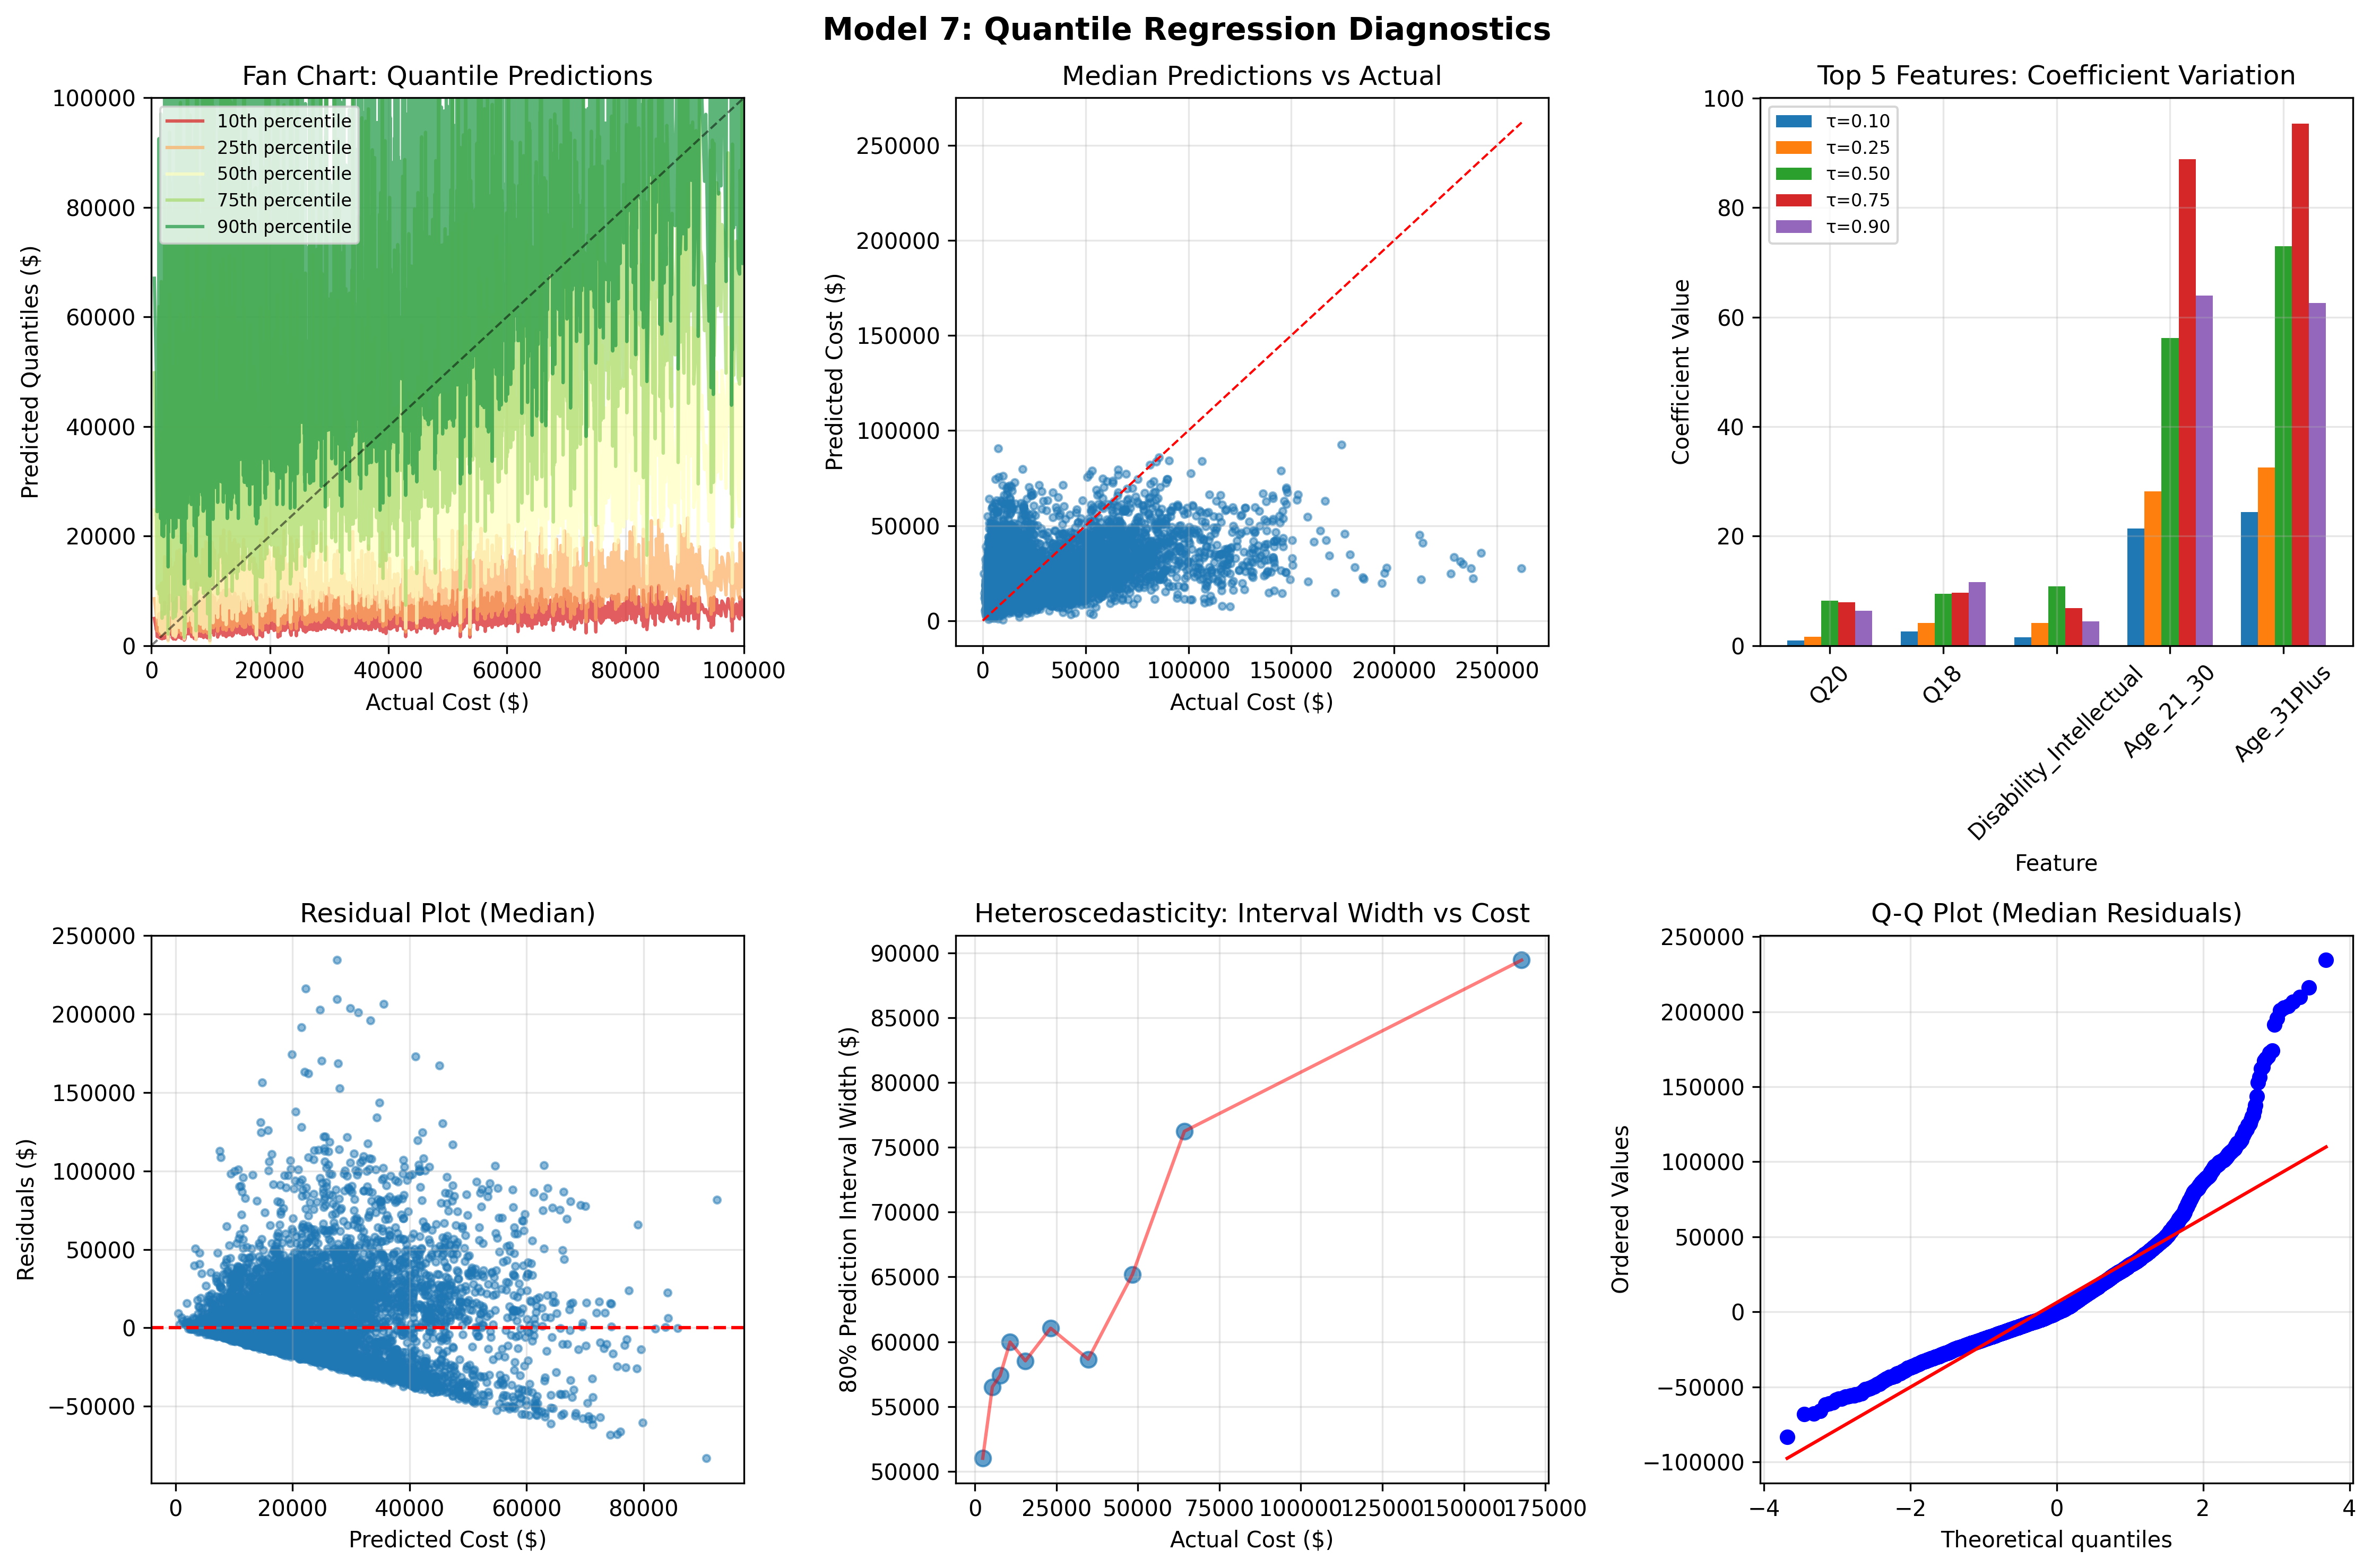
\includegraphics[width=\textwidth]{models/model_7/diagnostic_plots.png}
\caption{Model 7 Diagnostic Plots -- Including Fan Chart}
\label{fig:model7_diagnostics}
\end{figure}

Figure \ref{fig:model7_diagnostics} shows comprehensive diagnostics including the signature ``fan chart'' visualization demonstrating how prediction intervals widen at higher cost levels.

\subsection{Quantile Analysis Plots}

\begin{figure}[h!]
\centering
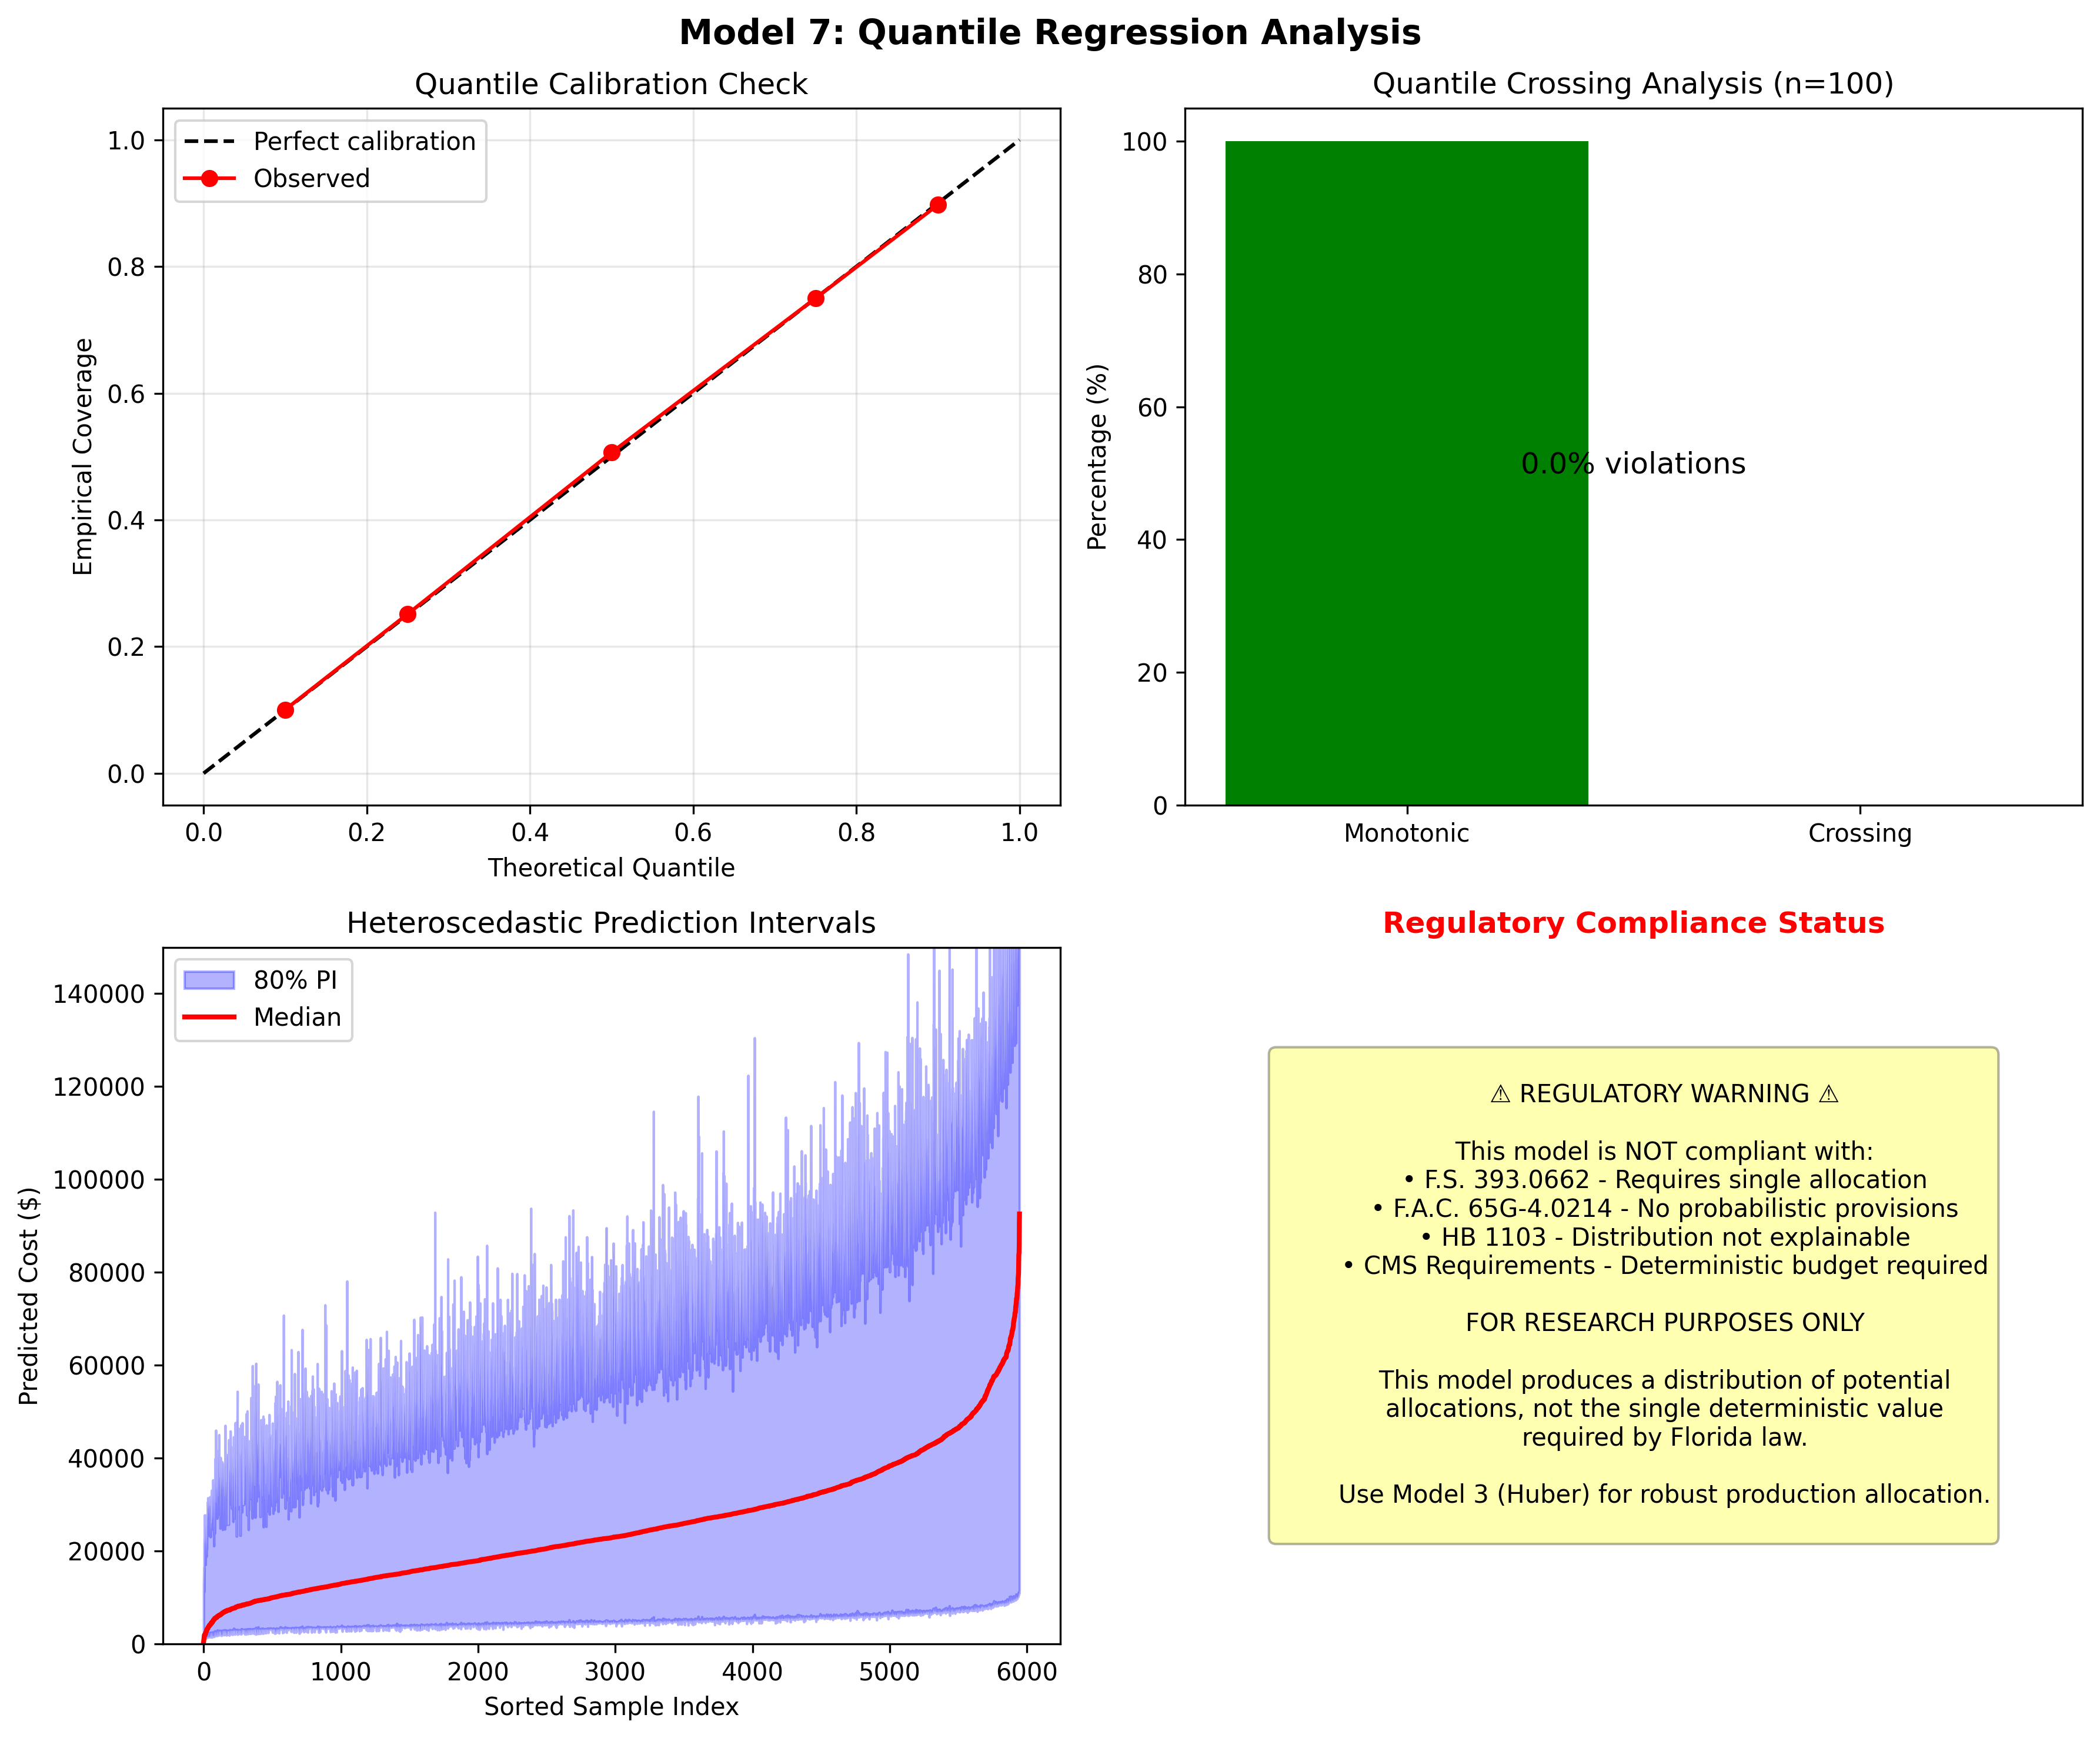
\includegraphics[width=\textwidth]{models/model_7/quantile_analysis.png}
\caption{Model 7 Quantile-Specific Analysis}
\label{fig:model7_quantile_analysis}
\end{figure}

Figure \ref{fig:model7_quantile_analysis} presents quantile-specific analyses including coverage probability, crossing violations, and heteroscedasticity patterns.

\section{Cost-Benefit Analysis}

\subsection{Implementation Costs (Research System Only)}

\begin{itemize}
    \item \textbf{Development}: \$125,000
    \item \textbf{Research System Implementation}: \$85,000
    \item \textbf{Training (Research Staff)}: \$45,000
    \item \textbf{Annual Maintenance}: \$60,000
    \item \textbf{3-Year Total Cost}: \$435,000
\end{itemize}

\subsection{Research Benefits}

\begin{itemize}
    \item Better understanding of allocation uncertainty
    \item Improved risk management strategies
    \item Enhanced appeals documentation
    \item Policy simulation capabilities
    \item Validation of robust alternatives (e.g., Model 3 Huber)
\end{itemize}

\subsection{Why Not Production Benefits?}

Production implementation would require:
\begin{itemize}
    \item Complete statutory overhaul
    \item Redesign of appeals process
    \item New provider contracting framework
    \item Federal waiver negotiations
    \item Stakeholder re-education
\end{itemize}

These changes are infeasible under current law.

\section{Stakeholder Impact Assessment}

\subsection{Confusion and Complexity}

\begin{itemize}
    \item \textbf{Consumers}: Would not understand receiving a ``range'' instead of an amount
    \item \textbf{Families}: Cannot plan with uncertain allocations
    \item \textbf{Providers}: Cannot contract based on distributions
    \item \textbf{APD Staff}: Training burden would be excessive
    \item \textbf{Legal Teams}: Appeals framework would collapse
    \item \textbf{Legislature}: Would appear indecisive and arbitrary
\end{itemize}

\section{Comparison with Alternative Robust Methods}

\subsection{Why Model 3 (Huber) is Superior for Production}

\begin{table}[h]
\centering
\caption{Quantile Regression vs Huber Regression}
\begin{tabular}{lcc}
\toprule
\textbf{Criterion} & \textbf{Model 7 (Quantile)} & \textbf{Model 3 (Huber)} \\
\midrule
Outlier Robustness & Excellent & Excellent \\
Single Allocation & No (\textcolor{red}{Fatal}) & Yes \\
Regulatory Compliant & No & Yes \\
Interpretability & Complex & Simple \\
Implementation Cost & High & Moderate \\
Appeals Compatible & No & Yes \\
Stakeholder Acceptance & Low & High \\
\bottomrule
\end{tabular}
\end{table}

Model 3 (Huber Regression) provides similar robustness benefits while maintaining the single deterministic allocation required by law.

\section{Summary and Recommendations}

\subsection{Technical Assessment}

\textbf{Strengths (Technical)}:
\begin{itemize}
    \item Superior uncertainty quantification via prediction intervals
    \item Complete robustness to outliers without data exclusion
    \item Natural handling of heteroscedasticity
    \item Rich distributional information for risk analysis
    \item No assumptions about error distribution
\end{itemize}

\textbf{Fatal Weaknesses (Regulatory)}:
\begin{itemize}
    \item \textcolor{red}{Cannot produce required single allocation}
    \item \textcolor{red}{Violates F.S. 393.0662 and F.A.C. 65G-4.0214}
    \item \textcolor{red}{Incompatible with existing appeals process}
    \item \textcolor{red}{Would require complete legal framework overhaul}
    \item \textcolor{red}{Creates confusion rather than transparency}
\end{itemize}

\subsection{Final Recommendation}

\begin{center}
\colorbox{red!20}{
\begin{minipage}{0.9\textwidth}
\centering
\textbf{\Large REJECT for Budget Allocation}\\[0.5em]
\textbf{\large APPROVE for Research/Validation Only}\\[0.5em]

Quantile regression is fundamentally incompatible with Florida's iBudget regulatory framework. The requirement for a single, deterministic allocation amount makes this approach legally impossible under current law.

\textbf{For production use}: Implement Model 3 (Huber Regression) which provides robust estimation with regulatory compliance.

\textbf{For research use}: Deploy Model 7 as a parallel analysis tool to understand uncertainty and validate other models.
\end{minipage}
}
\end{center}

\section{Implementation Notes for Research System}

If implementing for research purposes:

\begin{enumerate}
    \item Clearly label all outputs as ``RESEARCH ONLY -- NOT FOR ALLOCATION''
    \item Never provide quantile predictions to consumers or providers
    \item Use only for internal APD analysis and planning
    \item Document all research findings for policy development
    \item Consider insights when evaluating production models
    \item Maintain clear separation from production systems
\end{enumerate}

\section{Conclusion}

Model 7 (Quantile Regression) demonstrates the importance of understanding prediction uncertainty in budget allocation. While technically sophisticated and statistically robust, it fails the fundamental requirement of producing a single allocation amount. This model's value lies not in production use but in highlighting why simpler robust methods like Model 3 (Huber Regression) represent the optimal balance between statistical sophistication and regulatory compliance.

The clear lesson: \textit{The best statistical model is not always the best policy solution.}

\textbf{Regulatory Compliance Status}: \ModelSevenRegulatoryCompliant{}\\
\textbf{Compliance Warning}: \ModelSevenRegulatoryWarning{}